%% Chapter 11: PID Tuning Methods
%% IEEE-Formatted Control Systems Textbook
%% Self-contained chapter with complete derivations and practical experiments

\chapter{PID Tuning Methods}
\label{ch:pid_tuning}

\begin{quote}
\textit{``The problem of adjusting the constants of the automatic controller to give the best operation of the controlled equipment is one that has received much attention, but for which no general solution has been available.''}\\
\hfill --- Ziegler and Nichols, 1942
\end{quote}

%% ============================================================================
%% SECTION 1: HISTORICAL MOTIVATION
%% ============================================================================
\section{Historical Motivation: The Quest for Systematic Tuning}
\label{sec:pid_tuning_history}

\subsection{The Universal Problem of Controller Adjustment}

By the early 1940s, automatic controllers had become indispensable in industrial processes. The three-term PID controller, with its proportional, integral, and derivative actions, had emerged as the dominant architecture for feedback control. Yet a fundamental problem remained: how should an engineer determine the values of the controller gains $K_p$, $K_i$, and $K_d$?

Every industrial plant presented unique dynamics. A temperature controller for a chemical reactor behaved differently from a flow controller in a refinery, which in turn differed from a pressure controller in a boiler system. The transfer functions varied, the time constants ranged from milliseconds to hours, and the acceptable transient responses depended on the specific application. No single set of PID parameters could serve all purposes.

Before 1942, the art of controller tuning relied almost entirely on two approaches. The first was \textit{trial and error}, where operators would manually adjust gains while observing process behavior. This approach required significant experience and intuition. A skilled operator might eventually achieve satisfactory performance, but the process was time-consuming, potentially dangerous (oscillations in chemical processes could cause equipment damage or safety hazards), and the results were highly dependent on the individual's expertise. The second approach relied on \textit{expert knowledge}, where experienced control engineers developed ``rules of thumb'' for specific process types. These guidelines were passed down through apprenticeship and industrial experience. However, such knowledge was fragmented, inconsistent across industries, and often poorly documented.

The need for a systematic, scientific approach to controller tuning was acute. Industrial expansion during World War II accelerated this need, as factories required rapid commissioning with operators who lacked years of experience.

\subsection{Ziegler and Nichols: The First Systematic Methods (1942)}

\begin{historicalbox}[Ziegler and Nichols: Pioneers of Systematic PID Tuning]
In 1942, John G. Ziegler and Nathaniel B. Nichols, working at Taylor Instruments (later acquired by Honeywell), published their seminal paper ``Optimum Settings for Automatic Controllers'' in the \textit{Transactions of the ASME}. This work represented a watershed moment in control engineering, transforming controller tuning from an art requiring years of experience into a systematic procedure any trained operator could follow. Their methods, now known as the Ziegler-Nichols tuning rules, remain the foundation for industrial PID controller commissioning more than 80 years later.
\end{historicalbox}

This work represented a watershed moment in control engineering.

Ziegler and Nichols approached the problem empirically but systematically. They recognized that despite the diversity of industrial processes, certain measurable characteristics could be used to predict appropriate controller settings. Their key insight was that the \textit{dynamic response} of a process, rather than its detailed physics, contained sufficient information for controller tuning.

They proposed two distinct methods:

\paragraph{Method I: Process Reaction Curve (Open-Loop Method)}
This method applies to processes that exhibit a sigmoidal step response characteristic of self-regulating systems. By applying a step change to the manipulated variable and recording the process response, three parameters can be extracted: the process gain $K$, the apparent dead time $L$, and the dominant time constant $T$. From these three numbers, Ziegler and Nichols provided explicit formulas for $K_p$, $T_i$, and $T_d$.

\paragraph{Method II: Ultimate Gain Method (Closed-Loop Method)}
For processes where open-loop testing is impractical or unsafe, Ziegler and Nichols proposed a closed-loop procedure. With only proportional control active, the gain is gradually increased until the system exhibits sustained oscillations at the threshold of stability. The gain at this point ($K_u$, the ultimate gain) and the period of oscillation ($P_u$, the ultimate period) provide the information needed for tuning.

The beauty of these methods lay in their simplicity. An operator with minimal theoretical background could follow a straightforward procedure and obtain reasonable controller settings. The methods required no mathematical model of the process, no transfer function identification, and no complex calculations---only direct measurement of process behavior.

\subsection{The Design Philosophy: Quarter-Amplitude Damping}

Ziegler and Nichols designed their tuning rules to achieve a specific transient response: \textit{quarter-amplitude damping}. In this criterion, each successive oscillation peak is one-quarter the amplitude of the previous peak. Mathematically, for a step response, if the first overshoot is $A_1$ and the second overshoot is $A_2$, then:
\begin{equation}
    \frac{A_2}{A_1} = 0.25
\end{equation}

This corresponds to an effective damping ratio of approximately $\zeta \approx 0.21$ and results in roughly 25\% overshoot on the first peak. The quarter-amplitude criterion was chosen as a compromise because it provides reasonably fast response with short settling time, ensures that oscillations decay relatively quickly, and yields a response that is robust to modest parameter variations.

However, this aggressive tuning may be unsuitable for many applications. Processes where overshoot is unacceptable (such as positioning systems or certain chemical reactions) require more conservative tuning. This limitation, acknowledged by Ziegler and Nichols themselves, would later motivate the development of alternative methods.

\subsection{Cohen and Coon: Refinements for Self-Regulating Processes (1953)}

Despite the success of the Ziegler-Nichols methods, practitioners observed that the rules sometimes produced unsatisfactory results, particularly for processes with significant dead time relative to the time constant. In 1953, George H. Cohen and G. A. Coon, working at Foxboro Company, published improved tuning correlations specifically designed for self-regulating processes \cite{cohen1953}.

Cohen and Coon recognized that the ratio $\tau = L/T$ (normalized dead time) strongly influenced optimal controller settings. Their method, also based on the process reaction curve, incorporated this ratio explicitly into the tuning formulas. The Cohen-Coon rules generally provide better performance for processes with larger dead times ($\tau > 0.3$), reduced overshoot compared to Ziegler-Nichols, and improved robustness margins.

The Cohen-Coon method maintained the empirical, recipe-based philosophy of Ziegler-Nichols while offering enhanced accuracy for a broader class of processes.

\subsection{\AA{}str\"om and H\"agglund: Automatic Relay Tuning (1984)}

The next major advancement came four decades later when Karl Johan \AA{}str\"om and Tore H\"agglund at Lund University in Sweden introduced the \textit{relay feedback method} for automatic tuning \cite{astrom1984}.

Both Ziegler-Nichols methods had practical limitations. The open-loop method required taking the controller offline, which could disrupt production. Meanwhile, the closed-loop ultimate gain method required carefully increasing the gain to the stability boundary---a potentially dangerous procedure if the process was fast or if overshoot could cause damage.

\AA{}str\"om and H\"agglund's insight was elegant: instead of using a high-gain proportional controller to induce oscillations, use a \textit{relay} (on-off controller) in feedback. A relay controller is inherently nonlinear and will naturally create a limit cycle (sustained oscillation) without requiring careful gain adjustment.

The relay feedback test proceeds as follows.

\begin{algorithm}
\caption{Relay Feedback Auto-Tuning Procedure}
\begin{algorithmic}[1]
\State Replace the PID controller with a relay having output amplitude $d$ and hysteresis $\epsilon$
\State Close the feedback loop
\While{oscillations have not stabilized}
    \State Wait for the system to reach limit cycle behavior
\EndWhile
\State Measure the oscillation period $P_u$ and amplitude $a$
\State Calculate the ultimate gain: $K_u \gets 4d/(\pi a)$
\State Apply Ziegler-Nichols or other tuning rules using $K_u$ and $P_u$
\State \Return PID parameters $(K_p, T_i, T_d)$
\end{algorithmic}
\end{algorithm}

The relay method offered several advantages. The amplitude of oscillations is bounded by the relay amplitude $d$, ensuring safety. The test could be performed with the process near its operating point, and the procedure could be fully automated, requiring no operator intervention. Furthermore, the test duration was typically short, requiring only a few oscillation periods.

This innovation enabled the development of \textit{auto-tuning} controllers that could characterize the process and compute their own parameters. Such controllers became commercially available in the late 1980s and are now standard features in industrial DCS (Distributed Control System) platforms.

\subsection{The Continuing Need: From Operators to Algorithms}

The progression from Ziegler-Nichols through Cohen-Coon to relay auto-tuning reflects a consistent theme: the desire to remove human expertise from the loop. Each advancement reduced the knowledge required of the operator. With Ziegler-Nichols, one follows a procedure and calculates from formulas. Cohen-Coon uses improved formulas that handle more cases. Finally, relay auto-tuning requires only that the operator push a button and wait.

This evolution was driven by industrial reality. Process plants operate around the clock with rotating shifts. Not every operator has the experience to tune controllers manually. Equipment failures and process modifications require retuning. Commissioning new plants demands rapid startup.

Today, auto-tuning has become ubiquitous, embedded in everything from industrial distributed control systems to consumer thermostats. Yet the fundamental principles established by Ziegler and Nichols---extract process dynamics through simple tests, apply empirical correlations---remain the conceptual foundation for most tuning procedures.


%% ============================================================================
%% SECTION 2: MODERN APPLICATIONS
%% ============================================================================
\section{Modern Applications of PID Tuning Methods}
\label{sec:pid_tuning_modern}

The tuning methods developed in the mid-20th century have evolved into sophisticated tools embedded in modern control systems across diverse applications.

\subsection{Industrial Distributed Control Systems}

Modern DCS platforms from vendors such as Honeywell, Emerson, ABB, and Siemens include built-in auto-tuning functionality. These systems typically implement relay-based or step-response identification followed by automatic gain calculation. Advanced features include \textit{adaptive tuning}, which provides continuous monitoring of closed-loop performance with automatic gain adjustment when process dynamics change. \textit{Model-based tuning} enables identification of first-order-plus-dead-time (FOPDT) or second-order models with tuning based on specified performance objectives such as desired closed-loop time constant. \textit{Tuning wizards} offer guided procedures that walk operators through the tuning process with graphical displays of process response.

In modern refineries, chemical plants, and power generation facilities, thousands of PID loops operate simultaneously. Manual tuning of each loop is impractical; systematic auto-tuning is essential for efficient plant operation.

\subsection{Consumer and Commercial HVAC Systems}

Self-tuning thermostats represent one of the most widespread applications of automatic PID tuning. Modern ``smart'' thermostats from companies like Nest, Ecobee, and Honeywell implement adaptive algorithms that learn the thermal dynamics of a building. These systems identify heating and cooling time constants from observed temperature responses, adaptively adjust anticipation (derivative-like action) based on occupancy patterns, and optimize duty cycles to minimize energy consumption while maintaining comfort.

These systems apply the fundamental principle of Ziegler-Nichols---extract process dynamics, compute controller gains---using modern computational capabilities and machine learning enhancements.

\subsection{Unmanned Aerial Vehicles and Drones}

Multirotor drones require precise attitude control with PID controllers for roll, pitch, and yaw axes. Auto-tuning features are standard in flight controllers such as Betaflight, ArduPilot, and PX4. The tuning process typically involves automated oscillation tests on each axis, followed by identification of ultimate gain and frequency characteristics. The controller then computes PID gains with safety margins appropriate for flight, with iterative refinement based on pilot feedback.

The ``auto-tune'' mode in these flight controllers implements relay-like oscillation injection, measures the response, and calculates conservative PID parameters. This enables hobbyists without control engineering background to achieve stable flight.

\subsection{Software Tools: MATLAB/Simulink PID Tuner}

Modern control design software provides sophisticated interactive tuning tools. The MATLAB PID Tuner app exemplifies this capability. \textit{Model-based tuning} allows the software, given a plant transfer function or Simulink model, to compute optimal PID gains based on specified bandwidth and phase margin. \textit{Response visualization} through interactive sliders allows engineers to adjust response time and robustness while observing step response and frequency domain characteristics in real time. The software supports \textit{multiple design methods}, including Ziegler-Nichols, Cohen-Coon, IMC (Internal Model Control), and optimization-based methods. Finally, \textit{code generation} enables automatic generation of controller implementations for embedded systems.

These tools embody the accumulated wisdom of classical tuning methods while providing the computational power to optimize beyond what manual calculation could achieve.


%% ============================================================================
%% SECTION 3: MATHEMATICAL FOUNDATION
%% ============================================================================
\section{Mathematical Foundation}
\label{sec:pid_tuning_math}

We now develop the complete mathematical framework for the principal PID tuning methods. We consider a standard PID controller in the form:
\begin{equation}
    G_c(s) = K_p\left(1 + \frac{1}{T_i s} + T_d s\right)
\end{equation}
where $K_p$ is the proportional gain, $T_i$ is the integral time constant, and $T_d$ is the derivative time constant. The integral gain is $K_i = K_p/T_i$ and the derivative gain is $K_d = K_p T_d$.

\subsection{Process Characterization: The FOPDT Model}

Many industrial processes can be approximated by a \textit{First-Order Plus Dead-Time} (FOPDT) model:
\begin{equation}
    G_p(s) = \frac{K e^{-Ls}}{Ts + 1}
    \label{eq:fopdt}
\end{equation}
where $K$ denotes the process gain (steady-state gain), $T$ is the dominant time constant, and $L$ represents the apparent dead time (delay).

This model captures the essential dynamics of self-regulating processes: a delay before the response begins, followed by an exponential approach to a new steady state. The FOPDT approximation is remarkably effective for processes ranging from heat exchangers to chemical reactors to flow systems.

\subsection{Ziegler-Nichols Open-Loop Method (Process Reaction Curve)}

\subsubsection{Experimental Procedure}

The open-loop method requires recording the process response to a step change in the manipulated variable, as described in Algorithm~\ref{alg:open_loop_procedure}.

\begin{algorithm}
\caption{Ziegler-Nichols Open-Loop Experimental Procedure}
\label{alg:open_loop_procedure}
\begin{algorithmic}[1]
\State Bring the process to a stable operating point with the controller in manual mode
\State Apply a step change of magnitude $\Delta u$ to the manipulated variable
\State Record the process variable $y(t)$ as a function of time
\State Verify that the response exhibits a sigmoidal (S-shaped) curve characteristic of self-regulating processes
\State \Return Recorded process reaction curve $y(t)$
\end{algorithmic}
\end{algorithm}

\subsubsection{Parameter Extraction}

From the recorded process reaction curve, extract three parameters:

\paragraph{Process Gain ($K$):}
The ratio of the total change in the process variable to the step change in the manipulated variable:
\begin{equation}
    K = \frac{\Delta y}{\Delta u} = \frac{y(\infty) - y(0)}{u_{step}}
\end{equation}

\paragraph{Dead Time ($L$) and Time Constant ($T$):}
The classical graphical method involves drawing a tangent line at the inflection point of the S-curve (see Fig.~\ref{fig:process_reaction_curve}). The dead time $L$ is determined from the intersection of the tangent line with the initial value, representing the time at which the response ``begins.'' The quantity $L + T$ corresponds to the intersection of the tangent line with the final value, from which the time constant $T$ can be extracted.

Alternatively, the \textit{two-point method} uses the times at which the response reaches 28.3\% and 63.2\% of its final value:
\begin{equation}
    T = \frac{3}{2}\left(t_{63.2\%} - t_{28.3\%}\right), \qquad L = t_{63.2\%} - T
\end{equation}

\begin{figure}[htbp]
\centering
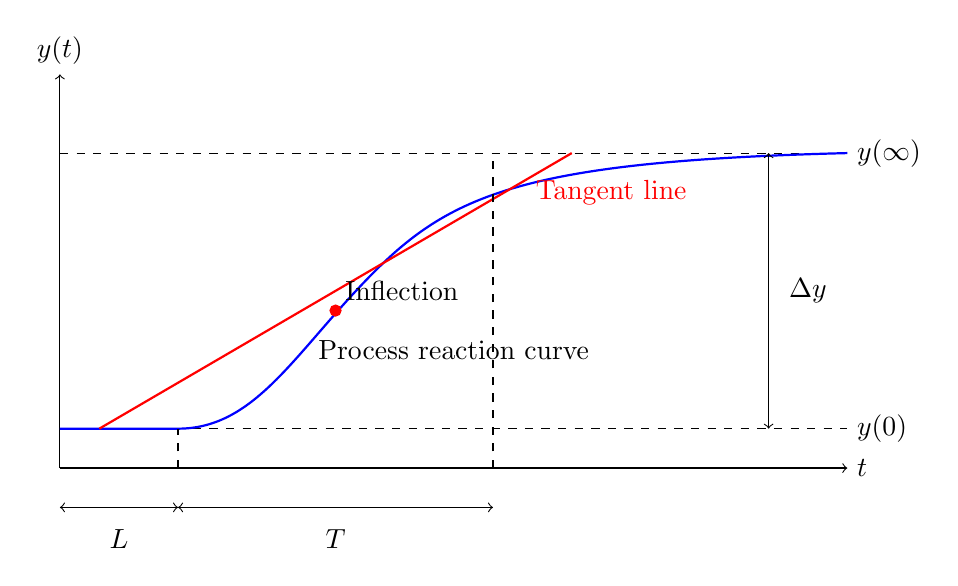
\begin{tikzpicture}[scale=1.0]
    % Axes
    \draw[->] (0,0) -- (10,0) node[right] {$t$};
    \draw[->] (0,0) -- (0,5) node[above] {$y(t)$};

    % Initial and final values
    \draw[dashed] (0,0.5) -- (10,0.5) node[right] {$y(0)$};
    \draw[dashed] (0,4) -- (10,4) node[right] {$y(\infty)$};

    % S-curve response
    \draw[thick, blue] (0,0.5) -- (1.5,0.5)
        .. controls (2.5,0.5) and (3,1.5) .. (4,2.5)
        .. controls (5,3.5) and (6,3.9) .. (10,4);

    % Tangent line at inflection point
    \draw[red, thick] (0.5,0.5) -- (6.5,4);

    % Dead time L
    \draw[<->] (0,-0.5) -- (1.5,-0.5);
    \node at (0.75,-0.9) {$L$};
    \draw[dashed] (1.5,0) -- (1.5,0.5);

    % Time constant T
    \draw[<->] (1.5,-0.5) -- (5.5,-0.5);
    \node at (3.5,-0.9) {$T$};
    \draw[dashed] (5.5,0) -- (5.5,4);

    % Delta y
    \draw[<->] (9,0.5) -- (9,4);
    \node at (9.5,2.25) {$\Delta y$};

    % Inflection point
    \filldraw[red] (3.5,2) circle (2pt);
    \node[above right] at (3.5,2) {Inflection};

    % Labels
    \node at (5,1.5) {Process reaction curve};
    \node[red] at (7,3.5) {Tangent line};
\end{tikzpicture}
\caption{Process reaction curve showing extraction of parameters $K$, $L$, and $T$. The dead time $L$ is the apparent delay before response begins. The time constant $T$ is found from the tangent at the inflection point.}
\label{fig:process_reaction_curve}
\end{figure}

\subsubsection{Ziegler-Nichols Open-Loop Tuning Rules}

From the extracted parameters, Ziegler and Nichols proposed the following tuning correlations:

\begin{table}[htbp]
\centering
\caption{Ziegler-Nichols Open-Loop (Process Reaction Curve) Tuning Rules}
\label{tab:zn_open_loop}
\begin{tabular}{lccc}
\toprule
\textbf{Controller} & $\boldsymbol{K_p}$ & $\boldsymbol{T_i}$ & $\boldsymbol{T_d}$ \\
\midrule
P & $\displaystyle\frac{T}{KL}$ & --- & --- \\[2ex]
PI & $\displaystyle\frac{0.9T}{KL}$ & $\displaystyle\frac{L}{0.3} = 3.33L$ & --- \\[2ex]
PID & $\displaystyle\frac{1.2T}{KL}$ & $2L$ & $0.5L$ \\
\bottomrule
\end{tabular}
\end{table}

\subsubsection{Derivation Rationale}

The Ziegler-Nichols rules can be understood through the following analysis. For a FOPDT process with the controller in the loop, the open-loop transfer function is:
\begin{equation}
    L(s) = G_c(s)G_p(s) = K_p\left(1 + \frac{1}{T_i s} + T_d s\right) \cdot \frac{K e^{-Ls}}{Ts + 1}
\end{equation}

For marginal stability, we require $|L(j\omega_c)| = 1$ and $\angle L(j\omega_c) = -180°$ at some critical frequency $\omega_c$. The dead time contributes phase $-\omega_c L$ radians.

The Ziegler-Nichols rules were derived empirically to place the closed-loop poles such that quarter-amplitude damping is achieved. The parameter $KL/T$ (normalized dead time times gain) is the key dimensionless group that determines the appropriate controller aggressiveness.

\subsection{Ziegler-Nichols Closed-Loop Method (Ultimate Gain)}

\subsubsection{Experimental Procedure}

The closed-loop method determines the stability boundary directly through the procedure described in Algorithm~\ref{alg:closed_loop_procedure}.

\begin{algorithm}
\caption{Ziegler-Nichols Closed-Loop (Ultimate Gain) Procedure}
\label{alg:closed_loop_procedure}
\begin{algorithmic}[1]
\State Configure the controller as P-only (set $T_i = \infty$, $T_d = 0$)
\State Close the feedback loop with a low value of $K_p$
\State Introduce a small setpoint change or disturbance
\While{oscillations are decaying or growing}
    \State Observe the transient response
    \State Increase $K_p$ by a small increment
\EndWhile
\State When sustained oscillations occur (constant amplitude), record:
\State \quad $K_u \gets$ current proportional gain (ultimate gain)
\State \quad $P_u \gets$ period of oscillation in seconds (ultimate period)
\State \Return $(K_u, P_u)$
\end{algorithmic}
\end{algorithm}

\begin{figure}[htbp]
\centering
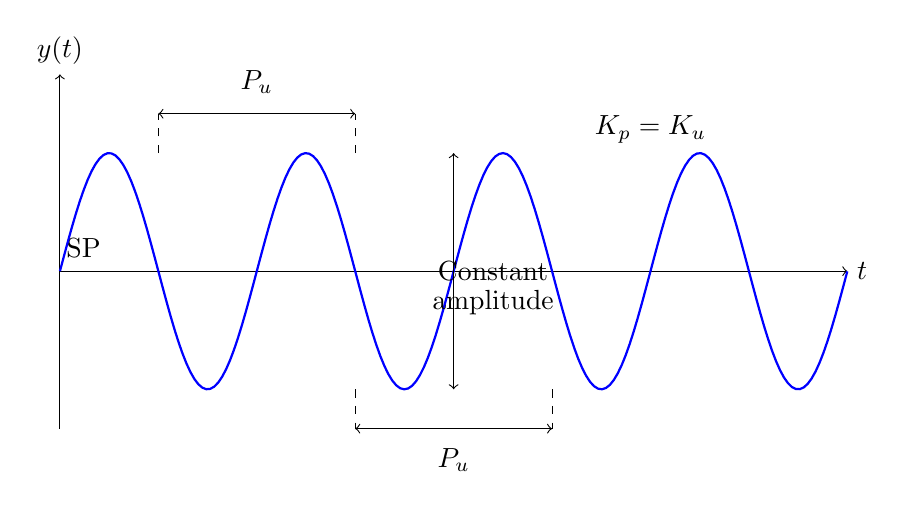
\begin{tikzpicture}[scale=1.0]
    % Axes
    \draw[->] (0,0) -- (10,0) node[right] {$t$};
    \draw[->] (0,-2) -- (0,2.5) node[above] {$y(t)$};

    % Setpoint
    \draw[dashed] (0,0) -- (10,0);
    \node at (0.3,0.3) {SP};

    % Sustained oscillation
    \draw[thick, blue, domain=0:10, samples=200]
        plot (\x, {1.5*sin(2*180*\x/2.5)});

    % Period marking
    \draw[<->] (1.25,2) -- (3.75,2);
    \node at (2.5,2.4) {$P_u$};

    % Amplitude marking
    \draw[<->] (5,-1.5) -- (5,1.5);
    \node at (5.5,0) {Constant};
    \node at (5.5,-0.4) {amplitude};

    % Second period marking
    \draw[<->] (3.75,-2) -- (6.25,-2);
    \node at (5,-2.4) {$P_u$};

    \draw[dashed] (1.25,1.5) -- (1.25,2);
    \draw[dashed] (3.75,1.5) -- (3.75,2);
    \draw[dashed] (3.75,-1.5) -- (3.75,-2);
    \draw[dashed] (6.25,-1.5) -- (6.25,-2);

    \node at (7.5,1.8) {$K_p = K_u$};
\end{tikzpicture}
\caption{Sustained oscillation at ultimate gain $K_u$ with period $P_u$. The oscillation amplitude remains constant, indicating the system is at the stability boundary.}
\label{fig:ultimate_oscillation}
\end{figure}

\subsubsection{Ziegler-Nichols Closed-Loop Tuning Rules}

\begin{table}[htbp]
\centering
\caption{Ziegler-Nichols Closed-Loop (Ultimate Gain) Tuning Rules}
\label{tab:zn_closed_loop}
\begin{tabular}{lccc}
\toprule
\textbf{Controller} & $\boldsymbol{K_p}$ & $\boldsymbol{T_i}$ & $\boldsymbol{T_d}$ \\
\midrule
P & $0.5 K_u$ & --- & --- \\[1ex]
PI & $0.45 K_u$ & $\displaystyle\frac{P_u}{1.2}$ & --- \\[2ex]
PID & $0.6 K_u$ & $\displaystyle\frac{P_u}{2}$ & $\displaystyle\frac{P_u}{8}$ \\
\bottomrule
\end{tabular}
\end{table}

\subsubsection{Theoretical Basis}

At the ultimate gain $K_u$, the closed-loop system has poles on the imaginary axis at $s = \pm j\omega_u$ where $\omega_u = 2\pi/P_u$. The Ziegler-Nichols rules move these poles into the left half-plane while introducing integral action (to eliminate steady-state error) and derivative action (to improve damping).

The factors in Table~\ref{tab:zn_closed_loop} can be understood as follows. Setting $K_p = 0.6 K_u$ means using 60\% of the ultimate gain, which provides a gain margin of $1/0.6 \approx 1.67$ or about 4.4~dB. The integral time constant $T_i = P_u/2$ is set to half the oscillation period, providing integral action without excessive phase lag at the critical frequency. The derivative time constant $T_d = P_u/8$ is one-quarter of the integral time, providing phase lead near the critical frequency.

\subsection{Cohen-Coon Method}

Cohen and Coon recognized that the Ziegler-Nichols rules could be improved by explicitly accounting for the normalized dead time $\tau = L/T$. Their tuning rules, derived from analysis of FOPDT processes, are:

\begin{table}[htbp]
\centering
\caption{Cohen-Coon Tuning Rules for FOPDT Processes}
\label{tab:cohen_coon}
\begin{tabular}{lc}
\toprule
\textbf{Parameter} & \textbf{Formula} \\
\midrule
$K_p$ & $\displaystyle\frac{1}{K}\cdot\frac{T}{L}\left(\frac{4}{3} + \frac{L}{4T}\right)$ \\[2ex]
$T_i$ & $\displaystyle L\cdot\frac{32 + 6L/T}{13 + 8L/T}$ \\[2ex]
$T_d$ & $\displaystyle L\cdot\frac{4}{11 + 2L/T}$ \\
\bottomrule
\end{tabular}
\end{table}

For the special case where $L \ll T$ (small dead time), the Cohen-Coon rules reduce approximately to:
\begin{equation}
    K_p \approx \frac{1.33T}{KL}, \quad T_i \approx 2.46L, \quad T_d \approx 0.36L
\end{equation}

Compared to Ziegler-Nichols PID ($K_p = 1.2T/(KL)$, $T_i = 2L$, $T_d = 0.5L$), Cohen-Coon provides slightly higher proportional gain, longer integral time (less aggressive integral action), and shorter derivative time.

These differences typically result in reduced overshoot and improved robustness, particularly for processes with significant dead time.

\subsection{Relay Feedback Auto-Tuning}

\subsubsection{The Relay Experiment}

The relay feedback method replaces the PID controller with an ideal relay:
\begin{equation}
    u(t) = \begin{cases}
        +d & \text{if } e(t) > 0 \\
        -d & \text{if } e(t) < 0
    \end{cases}
\end{equation}
where $d$ is the relay amplitude and $e(t) = r(t) - y(t)$ is the error signal.

\begin{figure}[htbp]
\centering
\begin{tikzpicture}[scale=0.9]
    % Block diagram
    \node[input] (input) {};
    \node[sum, right=of input] (sum) {};
    \node[block, right=of sum] (relay) {Relay};
    \node[block, right=2cm of relay] (process) {$G_p(s)$};
    \node[output, right=of process] (output) {};

    % Connections
    \draw[->] (input) -- node[above] {$r$} (sum);
    \draw[->] (sum) -- node[above] {$e$} (relay);
    \draw[->] (relay) -- node[above] {$u$} (process);
    \draw[->] (process) -- node[above] {$y$} (output);

    % Feedback
    \draw[->] (output) -- ++(0,-1.5) -| node[pos=0.9,left] {$-$} (sum);

    % Labels
    \node at (-0.5,0.3) {+};
    \node at (0,-0.5) {$-$};

    % Relay characteristic (inset)
    \begin{scope}[shift={(3,-3.5)}, scale=0.6]
        \draw[->] (-2,0) -- (2,0) node[right] {$e$};
        \draw[->] (0,-1.5) -- (0,1.5) node[above] {$u$};
        \draw[thick, blue] (-2,-1) -- (0,-1) -- (0,1) -- (2,1);
        \node at (1.2,1.3) {$+d$};
        \node at (1.2,-1.3) {$-d$};
    \end{scope}
\end{tikzpicture}
\caption{Relay feedback configuration for auto-tuning. The relay provides on-off control that naturally induces a limit cycle oscillation.}
\label{fig:relay_feedback}
\end{figure}

When a relay is placed in feedback with a process having sufficient phase lag, the system will naturally develop a \textit{limit cycle}---a sustained oscillation of fixed amplitude and period.

\subsubsection{Describing Function Analysis}

The relay can be analyzed using the \textit{describing function} method, which approximates the nonlinear element by its equivalent gain for sinusoidal inputs.

For an ideal relay with amplitude $d$ responding to a sinusoidal input $e(t) = a\sin(\omega t)$, the output is a square wave with amplitude $d$. The fundamental component of this square wave has amplitude:
\begin{equation}
    u_1 = \frac{4d}{\pi}
\end{equation}

The describing function (equivalent complex gain) is:
\begin{equation}
    N(a) = \frac{4d}{\pi a}
\end{equation}
where $a$ is the amplitude of the oscillation in the process output (error signal).

\subsubsection{Determination of Ultimate Gain and Period}

At the limit cycle, the describing function condition requires:
\begin{equation}
    N(a) \cdot G_p(j\omega) = -1
\end{equation}

This means:
\begin{equation}
    |G_p(j\omega_u)| = \frac{\pi a}{4d}, \qquad \angle G_p(j\omega_u) = -180°
\end{equation}

The ultimate gain is defined as $K_u = 1/|G_p(j\omega_u)|$, so:
\begin{equation}
    \boxed{K_u = \frac{4d}{\pi a}}
    \label{eq:relay_ku}
\end{equation}

The ultimate period is simply the observed period of oscillation:
\begin{equation}
    \boxed{P_u = \text{(measured oscillation period)}}
\end{equation}

\begin{examplebox}[Relay Auto-Tuning of a Heat Exchanger]
A temperature control system for a heat exchanger undergoes relay auto-tuning. The relay amplitude is set to $d = 5\%$ of valve range. After the system reaches limit cycle, the measured temperature oscillation has amplitude $a = 2.1\,^{\circ}\text{C}$ and period $P_u = 85\,\text{s}$.

\textbf{Solution:}

Calculate the ultimate gain using Equation~\eqref{eq:relay_ku}:
\begin{equation*}
K_u = \frac{4d}{\pi a} = \frac{4 \times 5}{\pi \times 2.1} = \frac{20}{6.60} = 3.03
\end{equation*}

Apply the Ziegler-Nichols closed-loop PID tuning rules from Table~\ref{tab:zn_closed_loop}:
\begin{align*}
K_p &= 0.6 \times K_u = 0.6 \times 3.03 = 1.82 \\
T_i &= \frac{P_u}{2} = \frac{85}{2} = 42.5\,\text{s} \\
T_d &= \frac{P_u}{8} = \frac{85}{8} = 10.6\,\text{s}
\end{align*}

These values provide a starting point. For reduced overshoot, $K_p$ might be reduced to 1.5 and $T_i$ increased to 50~s.
\end{examplebox}

\begin{examplebox}[Z-N Open-Loop Tuning from Step Response]
A level control process exhibits the following step response characteristics: process gain $K = 1.5\,\text{m}/\%$, apparent dead time $L = 12\,\text{s}$, and dominant time constant $T = 45\,\text{s}$. Determine the PID controller settings using the Ziegler-Nichols open-loop method.

\textbf{Solution:}

From Table~\ref{tab:zn_open_loop}, the PID tuning formulas are:
\begin{align*}
K_p &= \frac{1.2T}{KL} = \frac{1.2 \times 45}{1.5 \times 12} = \frac{54}{18} = 3.0 \\
T_i &= 2L = 2 \times 12 = 24\,\text{s} \\
T_d &= 0.5L = 0.5 \times 12 = 6\,\text{s}
\end{align*}

The normalized dead time ratio is $\tau = L/T = 12/45 = 0.27$, which is in the moderate range. These Z-N settings will likely produce approximately 25\% overshoot.
\end{examplebox}

\subsubsection{Practical Relay with Hysteresis}

In practice, a small hysteresis $\epsilon$ is added to prevent chattering due to noise:
\begin{equation}
    u(t) = \begin{cases}
        +d & \text{if } e(t) > +\epsilon \\
        -d & \text{if } e(t) < -\epsilon \\
        \text{previous value} & \text{otherwise}
    \end{cases}
\end{equation}

The describing function for a relay with hysteresis is:
\begin{equation}
    N(a,\epsilon) = \frac{4d}{\pi a}\sqrt{1 - \left(\frac{\epsilon}{a}\right)^2} - j\frac{4d}{\pi a}\cdot\frac{\epsilon}{a}
\end{equation}

For small hysteresis ($\epsilon \ll a$), the correction is negligible and Eq.~\eqref{eq:relay_ku} remains valid.

\subsection{Limitations of Classical Tuning Methods}

While Ziegler-Nichols and related methods have proven remarkably useful, they have well-documented limitations:

\paragraph{Quarter-Amplitude Damping:} The original Z-N rules target aggressive tuning with approximately 25\% overshoot. Many applications require tighter control (less overshoot) or cannot tolerate any overshoot.

\paragraph{Process Model Assumptions:} The methods assume the process can be reasonably approximated by an FOPDT model. Processes with significantly underdamped dynamics, inverse response, or multiple time constants may not be well-served.

\paragraph{Robustness:} The gain and phase margins achieved by Z-N tuning are modest. Process variations or modeling errors can lead to instability or poor performance.

\paragraph{Constrained Actuation:} The methods do not account for actuator saturation or rate limits, which are common in practice.

\paragraph{Noise Sensitivity:} Derivative action amplifies measurement noise. The derivative time $T_d = P_u/8$ from Z-N may be too aggressive for noisy processes.

For these reasons, Z-N and Cohen-Coon are often used as \textit{starting points}, with subsequent manual adjustment to meet specific performance requirements. Modern software tools provide optimization-based tuning that can better balance competing objectives.


%% ============================================================================
%% SECTION 4: PRACTICAL EXPERIMENT
%% ============================================================================
\section{Practical Experiment: Motor Speed Control Tuning}
\label{sec:pid_tuning_experiment}

\subsection{Objective}

In this experiment, you will apply the Ziegler-Nichols closed-loop method to tune a PID controller for DC motor speed regulation. You will then compare the Z-N settings with manually optimized gains.

\subsection{Required Equipment}

This experiment requires a DC motor with optical encoder (such as a Pololu 37D gearmotor with 64 CPR encoder), a motor driver (such as an L298N or TB6612FNG H-bridge), and an Arduino Mega or similar microcontroller. A power supply appropriate for the motor (typically 6--12~V) is needed, along with a computer running the Arduino IDE with Serial Plotter. An oscilloscope is optional but useful for precise timing measurements.

\subsection{System Setup}

The block diagram for the motor speed control system is shown in Fig.~\ref{fig:motor_control_block}.

\begin{figure}[htbp]
\centering
\begin{tikzpicture}[auto, node distance=2cm, >=latex']
    \node[input] (input) {};
    \node[sum, right=of input] (sum) {};
    \node[block, right=of sum] (pid) {PID};
    \node[block, right=of pid] (driver) {Driver};
    \node[block, right=of driver] (motor) {Motor};
    \node[output, right=of motor] (output) {};
    \node[block, below=1cm of motor] (encoder) {Encoder};

    \draw[->] (input) -- node {$\omega_{ref}$} (sum);
    \draw[->] (sum) -- node {$e$} (pid);
    \draw[->] (pid) -- node {PWM} (driver);
    \draw[->] (driver) -- node {$V$} (motor);
    \draw[->] (motor) -- node {$\omega$} (output);
    \draw[->] (encoder) -| node[pos=0.9] {$-$} (sum);
    \draw[->] (motor) |- (encoder);

    \node at (sum.south west) {$+$};
\end{tikzpicture}
\caption{Block diagram of motor speed control system for PID tuning experiment.}
\label{fig:motor_control_block}
\end{figure}

\subsection{Control Algorithm Framework}

The following algorithm describes the basic structure for the PID tuning experiment on a microcontroller.

\begin{algorithm}
\caption{Motor Speed PID Control Loop}
\label{alg:motor_pid}
\begin{algorithmic}[1]
\State \textbf{Initialize:}
\State \quad $K_p \gets 0$, $T_i \gets \infty$, $T_d \gets 0$ \Comment{Start with P-only control}
\State \quad $\text{setpoint} \gets 0$, $\text{integral} \gets 0$, $\text{prevError} \gets 0$
\State \quad $\Delta t \gets 0.01$ \Comment{Sample time in seconds}
\State \quad $\text{CPR} \gets 64$, $\text{GearRatio} \gets 30$ \Comment{Encoder and motor parameters}
\State Configure PWM output pins and encoder input pins
\State Enable encoder interrupt on rising edge
\State
\State \textbf{Encoder Interrupt Handler:}
\If{encoder channel B is high}
    \State $\text{encoderCount} \gets \text{encoderCount} + 1$
\Else
    \State $\text{encoderCount} \gets \text{encoderCount} - 1$
\EndIf
\State
\State \textbf{Main Control Loop:}
\While{system is running}
    \If{elapsed time $\geq \Delta t$}
        \State $\text{rpm} \gets \dfrac{(\text{encoderCount} - \text{prevCount}) \times 60}{\text{CPR} \times \text{GearRatio} \times \Delta t}$
        \State $\text{error} \gets \text{setpoint} - \text{rpm}$
        \State $\text{integral} \gets \text{integral} + \text{error} \times \Delta t$
        \State $\text{derivative} \gets \dfrac{\text{error} - \text{prevError}}{\Delta t}$
        \State $\text{output} \gets K_p \times \left(\text{error} + \dfrac{\text{integral}}{T_i} + T_d \times \text{derivative}\right)$
        \State $\text{prevError} \gets \text{error}$
        \State Apply PWM output with magnitude $|\text{output}|$ and appropriate direction
        \State Output setpoint and rpm for data logging
    \EndIf
\EndWhile
\end{algorithmic}
\end{algorithm}

\subsection{Procedure: Ziegler-Nichols Closed-Loop Method}

\subsubsection{Step 1: Determine Ultimate Gain and Period}

Follow Algorithm~\ref{alg:ultimate_gain_exp} to determine the ultimate gain and period experimentally.

\begin{algorithm}
\caption{Experimental Determination of Ultimate Gain}
\label{alg:ultimate_gain_exp}
\begin{algorithmic}[1]
\State Set $K_i \gets 0$ and $K_d \gets 0$ for P-only control
\State Set a moderate speed setpoint (e.g., 60 RPM)
\State Initialize $K_p \gets 0.1$
\While{oscillations are not sustained}
    \State Observe the response on the Serial Plotter
    \If{response is heavily damped (no oscillation)}
        \State $K_p \gets K_p \times 1.5$
    \EndIf
    \If{oscillations grow unbounded}
        \State Reduce $K_p$ immediately
    \EndIf
\EndWhile
\State Record $K_u \gets K_p$ (ultimate gain at sustained oscillation)
\State Record $P_u \gets$ measured peak-to-peak time (ultimate period)
\State \Return $(K_u, P_u)$
\end{algorithmic}
\end{algorithm}

\paragraph{Important:} If oscillations grow unbounded, reduce $K_p$ immediately. The ultimate gain is the \textit{maximum} gain for sustained oscillation.

\begin{table}[htbp]
\centering
\caption{Data Recording Template: Ultimate Gain Determination}
\label{tab:data_template}
\begin{tabular}{cccc}
\toprule
\textbf{Trial} & $\boldsymbol{K_p}$ & \textbf{Response Character} & \textbf{Notes} \\
\midrule
1 & 0.1 & Overdamped & No oscillation \\
2 & 0.15 & & \\
3 & 0.22 & & \\
4 & 0.33 & Underdamped & Oscillations decay \\
5 & 0.50 & & \\
6 & 0.75 & Critical & $K_u = $ \rule{1cm}{0.4pt}, $P_u = $ \rule{1cm}{0.4pt} s \\
\bottomrule
\end{tabular}
\end{table}

\subsubsection{Step 2: Calculate PID Gains}

Using the Ziegler-Nichols closed-loop formulas from Table~\ref{tab:zn_closed_loop}:

\begin{align}
    K_p &= 0.6 \times K_u = \rule{2cm}{0.4pt} \\
    T_i &= \frac{P_u}{2} = \rule{2cm}{0.4pt} \text{ s} \\
    T_d &= \frac{P_u}{8} = \rule{2cm}{0.4pt} \text{ s}
\end{align}

\subsubsection{Step 3: Test Z-N Parameters}

Enter the calculated $K_p$, $T_i$, and $T_d$ into the controller. Apply a step change in setpoint (e.g., 0 to 60 RPM) and record the step response using Serial Plotter. From the recorded response, measure the percent overshoot using $\%OS = (M_p - y_{ss})/y_{ss} \times 100\%$, the settling time based on the 2\% criterion, and the rise time from 10\% to 90\% of the final value.

\subsubsection{Step 4: Manual Fine-Tuning}

The Z-N settings typically produce aggressive response with significant overshoot. Fine-tune by first reducing $K_p$ by 20--30\% to decrease overshoot. If oscillations persist, increase $T_i$ by 50\%. If the system is too sensitive to noise, reduce $T_d$. Continue iterating through these adjustments until satisfactory performance is achieved.

\subsection{Results Template}

\begin{table}[htbp]
\centering
\caption{Comparison: Z-N Tuning vs Manual Optimization}
\label{tab:tuning_comparison}
\begin{tabular}{lccc}
\toprule
\textbf{Metric} & \textbf{Z-N Values} & \textbf{Manual Opt.} & \textbf{Units} \\
\midrule
$K_p$ & & & --- \\
$T_i$ & & & s \\
$T_d$ & & & s \\
\midrule
Percent Overshoot & & & \% \\
Settling Time & & & s \\
Rise Time & & & s \\
Steady-State Error & & & RPM \\
\bottomrule
\end{tabular}
\end{table}

\subsection{Discussion Questions}

Consider the following questions in your laboratory report. First, explain why the Z-N method produces approximately 25\% overshoot, relating this to the quarter-amplitude damping criterion. Second, discuss how the tuning would differ for a position control application where overshoot is unacceptable. Third, predict and explain what happens to the ultimate period as you add mechanical load to the motor. Finally, if you have collected open-loop step response data, compare your experimental results to what the Cohen-Coon method would predict.


%% ============================================================================
%% SECTION 5: EXAMPLE PROBLEMS
%% ============================================================================
\section{Example Problems}
\label{sec:pid_tuning_examples}

\subsection{Example 11.1: Extracting FOPDT Parameters from Process Reaction Curve}

\paragraph{Problem:} A step change of $\Delta u = 5\%$ is applied to a valve in a temperature control loop. The recorded process response is shown below. The initial temperature was $150°C$ and the final temperature is $162°C$. From the tangent at the inflection point, the line intersects $150°C$ at $t = 8$ s and intersects $162°C$ at $t = 32$ s. Determine the FOPDT model parameters $K$, $L$, and $T$.

\paragraph{Solution:}

\textbf{Step 1: Calculate Process Gain}
\begin{equation}
    K = \frac{\Delta y}{\Delta u} = \frac{162 - 150}{5\%} = \frac{12°C}{5\%} = 2.4 \text{ °C/\%}
\end{equation}

\textbf{Step 2: Determine Dead Time}

The tangent line intersects the initial value at $t = 8$ s:
\begin{equation}
    L = 8 \text{ s}
\end{equation}

\textbf{Step 3: Determine Time Constant}

The tangent line intersects the final value at $t = 32$ s:
\begin{equation}
    T = 32 - 8 = 24 \text{ s}
\end{equation}

\textbf{FOPDT Model:}
\begin{equation}
    G_p(s) = \frac{2.4 \, e^{-8s}}{24s + 1}
\end{equation}

\textbf{Check:} The normalized dead time is $\tau = L/T = 8/24 = 0.33$, which is within the typical range for self-regulating processes.

\hrulefill

\subsection{Example 11.2: Ziegler-Nichols Open-Loop Tuning}

\paragraph{Problem:} Using the FOPDT parameters from Example 11.1 ($K = 2.4$, $L = 8$ s, $T = 24$ s), calculate the PID controller settings using the Ziegler-Nichols open-loop method.

\paragraph{Solution:}

From Table~\ref{tab:zn_open_loop}:

\textbf{Proportional Gain:}
\begin{equation}
    K_p = \frac{1.2 T}{K L} = \frac{1.2 \times 24}{2.4 \times 8} = \frac{28.8}{19.2} = 1.5
\end{equation}

\textbf{Integral Time:}
\begin{equation}
    T_i = 2L = 2 \times 8 = 16 \text{ s}
\end{equation}

\textbf{Derivative Time:}
\begin{equation}
    T_d = 0.5L = 0.5 \times 8 = 4 \text{ s}
\end{equation}

\textbf{Complete PID Controller:}
\begin{equation}
    G_c(s) = 1.5\left(1 + \frac{1}{16s} + 4s\right)
\end{equation}

Or in parallel form: $K_p = 1.5$, $K_i = K_p/T_i = 0.094$ s$^{-1}$, $K_d = K_p T_d = 6$ s.

\hrulefill

\subsection{Example 11.3: Ziegler-Nichols Closed-Loop Tuning}

\paragraph{Problem:} A closed-loop experiment on a pressure control system yields the following results. With proportional-only control, sustained oscillations occur at $K_p = 8.5$ with an oscillation period of $1.6$ s. Calculate the PID settings using the Z-N closed-loop method.

\paragraph{Solution:}

Given: $K_u = 8.5$, $P_u = 1.6$ s

From Table~\ref{tab:zn_closed_loop}:

\textbf{Proportional Gain:}
\begin{equation}
    K_p = 0.6 K_u = 0.6 \times 8.5 = 5.1
\end{equation}

\textbf{Integral Time:}
\begin{equation}
    T_i = \frac{P_u}{2} = \frac{1.6}{2} = 0.8 \text{ s}
\end{equation}

\textbf{Derivative Time:}
\begin{equation}
    T_d = \frac{P_u}{8} = \frac{1.6}{8} = 0.2 \text{ s}
\end{equation}

\textbf{Complete PID Controller:}
\begin{equation}
    G_c(s) = 5.1\left(1 + \frac{1}{0.8s} + 0.2s\right)
\end{equation}

\hrulefill

\subsection{Example 11.4: Comparing Ziegler-Nichols and Cohen-Coon}

\paragraph{Problem:} For the process in Example 11.1 ($K = 2.4$, $L = 8$ s, $T = 24$ s), calculate the PID settings using the Cohen-Coon method and compare with the Z-N results.

\paragraph{Solution:}

First, calculate the normalized dead time:
\begin{equation}
    \tau = \frac{L}{T} = \frac{8}{24} = 0.333
\end{equation}

\textbf{Cohen-Coon Proportional Gain:}
\begin{align}
    K_p &= \frac{1}{K}\cdot\frac{T}{L}\left(\frac{4}{3} + \frac{L}{4T}\right) \\
    &= \frac{1}{2.4}\cdot\frac{24}{8}\left(\frac{4}{3} + \frac{8}{4 \times 24}\right) \\
    &= \frac{1}{2.4} \times 3 \times \left(1.333 + 0.083\right) \\
    &= 1.25 \times 1.417 = 1.77
\end{align}

\textbf{Cohen-Coon Integral Time:}
\begin{align}
    T_i &= L \cdot \frac{32 + 6(L/T)}{13 + 8(L/T)} \\
    &= 8 \times \frac{32 + 6(0.333)}{13 + 8(0.333)} \\
    &= 8 \times \frac{32 + 2}{13 + 2.67} \\
    &= 8 \times \frac{34}{15.67} = 17.4 \text{ s}
\end{align}

\textbf{Cohen-Coon Derivative Time:}
\begin{align}
    T_d &= L \cdot \frac{4}{11 + 2(L/T)} \\
    &= 8 \times \frac{4}{11 + 2(0.333)} \\
    &= 8 \times \frac{4}{11.67} = 2.74 \text{ s}
\end{align}

\textbf{Comparison:}
\begin{table}[htbp]
\centering
\begin{tabular}{lccc}
\toprule
\textbf{Parameter} & \textbf{Z-N} & \textbf{Cohen-Coon} & \textbf{Difference} \\
\midrule
$K_p$ & 1.5 & 1.77 & +18\% \\
$T_i$ & 16 s & 17.4 s & +9\% \\
$T_d$ & 4 s & 2.74 s & $-31\%$ \\
\bottomrule
\end{tabular}
\end{table}

Cohen-Coon gives higher proportional gain, longer integral time (less aggressive integral action), and shorter derivative time. For this process with moderate dead time ($\tau = 0.33$), the differences are meaningful. Cohen-Coon will typically produce less overshoot and better robustness.

\hrulefill

\subsection{Example 11.5: Relay Auto-Tuning Analysis}

\paragraph{Problem:} A relay with amplitude $d = 5\%$ is placed in feedback with a flow control process. After the system reaches a limit cycle, the flow measurement oscillates between 47.2 and 52.8 units with a period of 3.4 s. Calculate the ultimate gain and ultimate period, then determine Z-N PID settings.

\paragraph{Solution:}

\textbf{Step 1: Determine Oscillation Amplitude}

The peak-to-peak amplitude is $52.8 - 47.2 = 5.6$ units.
The amplitude $a$ (half of peak-to-peak) is:
\begin{equation}
    a = \frac{52.8 - 47.2}{2} = 2.8 \text{ units}
\end{equation}

\textbf{Step 2: Calculate Ultimate Gain}

Using Eq.~\eqref{eq:relay_ku}:
\begin{equation}
    K_u = \frac{4d}{\pi a} = \frac{4 \times 5}{\pi \times 2.8} = \frac{20}{8.80} = 2.27
\end{equation}

\textbf{Step 3: Record Ultimate Period}
\begin{equation}
    P_u = 3.4 \text{ s}
\end{equation}

\textbf{Step 4: Calculate Z-N PID Settings}
\begin{align}
    K_p &= 0.6 K_u = 0.6 \times 2.27 = 1.36 \\
    T_i &= \frac{P_u}{2} = \frac{3.4}{2} = 1.7 \text{ s} \\
    T_d &= \frac{P_u}{8} = \frac{3.4}{8} = 0.425 \text{ s}
\end{align}

\hrulefill

\subsection{Example 11.6: Effect of Process Uncertainty}

\paragraph{Problem:} A process is nominally characterized by $K = 1.0$, $L = 2$ s, $T = 10$ s. Z-N open-loop tuning gives $K_p = 6$, $T_i = 4$ s, $T_d = 1$ s. If the actual process has 20\% higher gain ($K = 1.2$), analyze the effect on stability.

\paragraph{Solution:}

\textbf{Nominal Design:}

The open-loop transfer function at the crossover frequency can be analyzed. The Z-N method targets a gain margin of approximately $1/0.6 \approx 1.67$ (4.4 dB).

\textbf{Effect of Gain Increase:}

If the process gain increases by 20\%, the loop gain increases proportionally. The effective loop gain becomes:
\begin{equation}
    \text{New loop gain} = \frac{1.2}{1.0} \times K_p = 1.2 \times 6 = 7.2
\end{equation}

relative to the nominal design.

\textbf{Stability Analysis:}

The Z-N design had gain margin of $20\log_{10}(1.67) = 4.4$ dB. The 20\% gain increase corresponds to:
\begin{equation}
    20\log_{10}(1.2) = 1.6 \text{ dB}
\end{equation}

The remaining gain margin is:
\begin{equation}
    4.4 - 1.6 = 2.8 \text{ dB}
\end{equation}

The system remains stable but with reduced robustness. The response will exhibit more overshoot and longer settling time than nominal.

\textbf{Conclusion:} Z-N tuning provides modest robustness margins. For processes with significant uncertainty, more conservative tuning (e.g., reducing $K_p$ by 20--30\%) is recommended.


%% ============================================================================
%% SECTION 6: SUMMARY AND REFERENCES
%% ============================================================================
\section{Chapter Summary}

This chapter presented the classical methods for PID controller tuning. The \textit{historical context} establishes that Ziegler and Nichols (1942) introduced the first systematic tuning methods, transforming controller adjustment from an art to a science. The \textit{Ziegler-Nichols open-loop method} extracts parameters $K$, $L$, and $T$ from a step response and applies the formulas in Table~\ref{tab:zn_open_loop}. The \textit{Ziegler-Nichols closed-loop method} determines $K_u$ and $P_u$ by increasing proportional gain to sustained oscillation, then applies Table~\ref{tab:zn_closed_loop}. The \textit{Cohen-Coon method} provides improved formulas that account for the normalized dead time ratio $L/T$. \textit{Relay auto-tuning} uses a relay in feedback to safely induce oscillations, calculating $K_u = 4d/(\pi a)$ from the limit cycle. Finally, it is important to recognize the \textit{limitations} of these classical methods: they target quarter-amplitude damping (25\% overshoot) and provide modest robustness margins, serving primarily as starting points for further optimization.

\section*{Key Equations}

\begin{align}
    \text{FOPDT Model:} \quad G_p(s) &= \frac{K e^{-Ls}}{Ts + 1} \\[1ex]
    \text{Z-N Open-Loop PID:} \quad K_p &= \frac{1.2T}{KL}, \quad T_i = 2L, \quad T_d = 0.5L \\[1ex]
    \text{Z-N Closed-Loop PID:} \quad K_p &= 0.6K_u, \quad T_i = \frac{P_u}{2}, \quad T_d = \frac{P_u}{8} \\[1ex]
    \text{Relay Ultimate Gain:} \quad K_u &= \frac{4d}{\pi a}
\end{align}

\newpage
\section{Exercises}

\begin{exercise}
A process has the transfer function $G(s) = \frac{2.5 e^{-3s}}{15s+1}$. Calculate the PID parameters using both Z-N open-loop and Cohen-Coon methods. Compare the results and explain any differences.
\end{exercise}

\begin{exercise}
An ultimate gain test yields $K_u = 12$ and $P_u = 0.8$ s. Calculate PI and PID settings using the Z-N closed-loop method.
\end{exercise}

\begin{exercise}
A relay with $d = 10\%$ produces oscillations with amplitude $a = 4\%$ and period $P_u = 2.5$ s. Find $K_u$ and the Z-N PID settings.
\end{exercise}

\begin{exercise}
Explain why the Cohen-Coon method reduces the derivative time $T_d$ compared to Z-N for processes with large dead time.
\end{exercise}

\begin{exercise}
A temperature process has $K = 0.8$ °C/\%, $L = 45$ s, and $T = 180$ s. (a) Calculate Z-N PID settings. (b) If the acceptable overshoot is 10\%, suggest modifications to the Z-N gains.
\end{exercise}

\begin{exercise}
For the relay auto-tuning method, derive the relationship between relay hysteresis $\epsilon$ and the phase angle of the describing function.
\end{exercise}

\begin{exercise}
A motor speed control system has $K_u = 5.2$ and $P_u = 0.12$ s. (a) Calculate Z-N PID gains. (b) Calculate the corresponding natural frequency and damping ratio of the closed-loop poles.
\end{exercise}

\begin{exercise}
Compare the gain margins achieved by P, PI, and PID controllers tuned using the Z-N closed-loop method.
\end{exercise}

\begin{exercise}
A chemical reactor has a first-order-plus-dead-time model with $K = 2.0$, $L = 8$ min, and $T = 20$ min. Calculate the normalized dead time ratio $\tau = L/T$. Is this process more suitable for Z-N or Cohen-Coon tuning? Calculate both sets of PID parameters.
\end{exercise}

\begin{exercise}
During relay auto-tuning of a pressure control loop, the relay amplitude is $d = 5\%$ and hysteresis is $\epsilon = 0.5\%$. The observed oscillation has amplitude $a = 3.2\%$ and period $P_u = 4.5$ s. Calculate the corrected ultimate gain accounting for hysteresis.
\end{exercise}

\begin{exercise}
Derive the quarter-amplitude damping criterion mathematically. Show that this corresponds to an effective damping ratio of approximately $\zeta \approx 0.21$.
\end{exercise}

\begin{exercise}
Design and conduct a relay auto-tuning experiment on a simulated or physical first-order system. Document your procedure, measurements, and resulting PID parameters. Verify the performance through step response testing.
\end{exercise}

\begin{thebibliography}{9}

\bibitem{ziegler1942}
J. G. Ziegler and N. B. Nichols, ``Optimum settings for automatic controllers,'' \textit{Trans. ASME}, vol. 64, no. 11, pp. 759--768, 1942.

\bibitem{cohen1953}
G. H. Cohen and G. A. Coon, ``Theoretical consideration of retarded control,'' \textit{Trans. ASME}, vol. 75, pp. 827--834, 1953.

\bibitem{astrom1984}
K. J. \AA{}str\"om and T. H\"agglund, ``Automatic tuning of simple regulators with specifications on phase and amplitude margins,'' \textit{Automatica}, vol. 20, no. 5, pp. 645--651, 1984.

\bibitem{astrom1995}
K. J. \AA{}str\"om and T. H\"agglund, \textit{PID Controllers: Theory, Design, and Tuning}, 2nd ed. Research Triangle Park, NC: ISA, 1995.

\bibitem{oconnor2003}
D. O'Dwyer, \textit{Handbook of PI and PID Controller Tuning Rules}. London: Imperial College Press, 2003.

\bibitem{seborg2011}
D. E. Seborg, T. F. Edgar, D. A. Mellichamp, and F. J. Doyle III, \textit{Process Dynamics and Control}, 3rd ed. Hoboken, NJ: Wiley, 2011.

\end{thebibliography}
